\documentclass[11pt,oneside]{scrbook}
 \usepackage[ngerman]{babel}
\usepackage[applemac]{inputenc}
\usepackage[T1]{fontenc}
\usepackage{supertabular}
\usepackage{graphicx}
%\usepackage{flafter}
\usepackage{hyperref}
\renewcommand{\familydefault}{\sfdefault}
\usepackage{helvet}
\usepackage{rotating}
\usepackage[final]{pdfpages}
%\usepackage{hyperref}
\usepackage{listings}
\usepackage{supertabular}


%\setcounter{tocdepth}{3}
%\setcounter{secnumdepth}{3}
%\lstset{language=Perl}
\lstset{tabsize=2}
\lstset{frame=plain}

\setcounter{tocdepth}{1}

\begin{document}
{
\centering
%
\includegraphics[scale=0.2]{figs/logo.PNG}

~\\ 

{\noindent \huge \bf CapClinical \\~\\}
{\noindent \large \bf Clinical trials in a box\\~\\}
{\noindent   Daniel Bšhringer}

}
\tableofcontents
\newpage

\chapter{Einleitung}
\section{Ziele  des Programmes}
GrundsŠtzliches Ziel ist der barrierefreie Zugriff auf alle zur DurchfŸhrung einer klinischen Studie erforderlichen Informationen ermšglichen. ZusŠtzlich sollen redundante Dateneingaben konsequent vermieden werden ('don't repeat yourself', beispielsweise automatische "Ubernahme aller Visitentermine in den †bersichtskalender, die MerkblŠtter, die Fahrtkostenabrechnungen und in die Sponsorrechnungen). Schlussendlich  soll auch die Quelldatendokumentation erleichtert werden.


Durch die Realisation des Programmes als Web-Anwendung ist es von jedem Bildschirmarbeitsplatz  ohne Softwareinstallation verfŸgbar. Das Programm lŠuft in allen aktuellen Browsern (Safari, Chrome, Firefox und Internet Explorer).
Das leistungsstarke Framework Cappuccino (www.cappuccino.org) ermšglicht dabei alle Funktionen  klassischer Computerprogramme, wie z.B. Tastatursteuerung, Copy/Paste sowie Undo und Redo.

\section{Grundlegende Bedinungskonzepte}
\label{ui-concepts}
Ein zentrales Element in der BenutzeroberflŠche ist das so genannte {\it TableView} (Abbildung \ref{fig:tableView}). Die Zeilen einer solchen Tabelle kšnnen selektiert sein und sind dann invertiert (wei§e Schrift auf dunklem Hintergrund). Eine Zeile wird mit einem einem einfachen Mausklick selektiert. In diesem Fall wird die vorherige Selektion annulliert. Ist wŠhrend des Mausklicks die Shift- bzw. Kommando-Taste gedrŸckt, wird die  vorhandene Selektion nicht annuliert, sondern die angeklickte Zeile zusŠtzlich markiert. Mit gedrŸckter Kommando-Taste kann eine selektierte Zeile auch gezielt deselektiert und die restliche Selektion  erhalten werden. Die Selektion ist Grundlage fŸr Aktionen aus dem 'ButtonBar' unterhalb der Tabelle (Abbildung \ref{fig:tableView}). Der Minus-Knopf lšscht die selektierten Zeilen, der Plus-Knopf generiert eine neue Zeile. †ber den 'Zahnrad'-Knopf sind weitere Aktionen auf die selektieren Zeilen zugŠnglich. Ggf. sind zusŠtzlch Aktionsknšpfe mit Piktogrammen neben dem ZahnradmenŸ aufgereiht. Eine Kurzbeschreibung ('Tool tip') dieser Aktionen erscheint wenn der Mauszeiger eine kurze Zeit Ÿber den Knopf positioniert wird. Endet der 'Tool tip' mit drei Punkten, erfolgt nach dem DrŸcken der SchaltflŠche noch eine RŸckfrage.

\begin{figure}[htbp]
\begin{center}
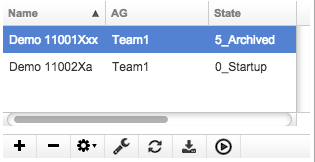
\includegraphics[scale=0.8]{figs/tableview.png}
\caption{Das so genannte {\it TableView} ist ein immer wiederkehrendes Element in der BenutzeroberflŠche. Die Spalten lassen sich sortieren, in der Breite Šndern und verschieben. Darunter befindet sich in der Regel ein {\it ButtonBar} fŸr Aktionen auf die Daten der Tabelle.}
\label{fig:tableView}
\end{center}
\end{figure}

Ein Klick auf die TabellenŸberschrift sortiert die Tabelle nach der angeklickten Spalte. Spalten lassen sich durch klicken und ziehen umsortieren. Die Breite von Tabellenspalten lŠsst sich durch Ziehen des Spaltenzwischenraumes anpassen. Diese €nderungen werden lokal gespeichert und bei einem neuen Programmaufruf wiederhergestellt.
In der Regel ermšglicht ein Doppelklick auf das TableView das Bearbeiten der angeklickten Zelle. Ggf. šffnen sich spezifische Eingabehilfen wie ein Mini-Kalender.


\chapter{StudienŸbersicht}
Die StudienŸbersicht befindet sich in der linken Spalte der BenutzeroberflŠche (Abbildung \ref{fig:uebersicht}). Die Breite der linken Spalte lŠsst sich durch Ziehen der dŸnnen schwarzen Trennlinie rechts neben dem TableView (dauerhaft) anpassen. Neben Studientitel und zugewiesener Arbeitsgruppe findet sich der momentane Stand im 'Lebenszyklus' der Studie, die Studienphase sowie der Sponsor in der Tabelle. Nur der Studientitel ist Ÿber Doppelklick direkt editierbar. Der Studienstand ermittelt sich automatisch aus Angaben im Bereich 'Zeitereignisse' (s. Kapitel \ref{section:zyklus}). Die  Studienphase und der Sponsor werden  automatisch den entsprechenden Angaben der strukturierten Datenablage entnommen, und mŸssen ggf. an dieser Stelle verŠndert werden (s. Kapitel \ref{chap:data}).

\begin{figure}[htbp]
\begin{center}
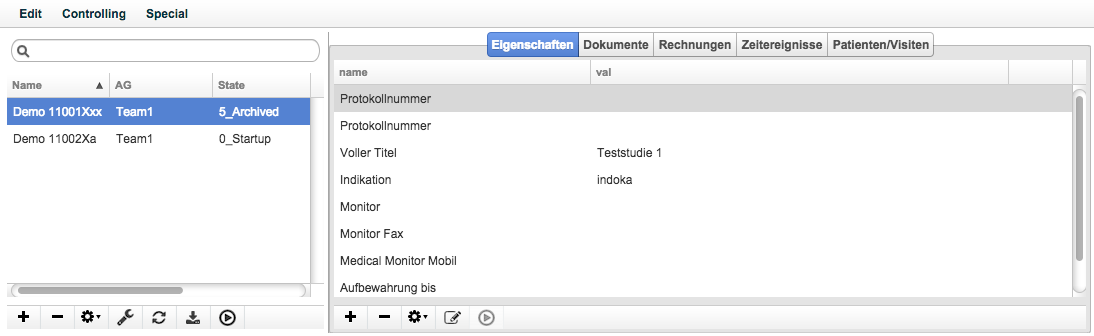
\includegraphics[scale=0.38]{figs/overview.png}
\caption{Die BenutzeroberflŠche unterteilt sich in einen konstanten linken Bereich mit der StudienŸbersicht und einen variablen rechten Bereich, dessen Inhalt Ÿber die Tab-Reiter im Kopfbereich bestimmt wird. Die Breite des linken und rechten Bereiches lŠsst sich Ÿber das Ziehen der Trennlinie mit der Maus jederzeit verŠndern.}
\label{fig:uebersicht}
\end{center}
\end{figure}

†ber der StudienŸbersicht befindet sich ein Suchfeld, dass wŠhrend  der Eingabe kontinuierlich die Studienliste auf die Suchtreffer reduziert. Dabei werden  neben dem Titel der Studie auch alle Felder der strukturierten Datenablage und alle Namen der eingeschlossenen Patienten durchsucht.

Die selektierte Studie kann Ÿber den Minus-Knopf des ButtonBars unter der Studienliste gelšscht werden. †ber das ZahnradmenŸ lassen sich ausgefŸllte Formulare fŸr die selektierte Studie abrufen  (momentan nur Drittmittelanzeige und allgemeines Vertragsanschreiben).

Der 'Reload-Knopf' frischt die Studientabelle auf. Dies ist insbesondere nach €nderungen in den Zeitereignissen sinnvoll, die den Studienstatus beeinflussen. Der Download Knopf lŠdt eine Excel-Tabelle mit allen sichtbaren Studien herunter. Der Play-Knopf šffnet eine eingegrenzte Eingabemaske auf die selektierte Studie.

\section{Neue Studie anlegen und konfigurieren}
Eine neue Studie wird auf den Plus-Knopf des ButtonBars unter der Studienliste generiert. Die Studie wird dabei automatisch der ersten Arbeitsgruppe des angemeldeten Benutzers zugeordnet. Direkt nach dem Anlegen wird  der Eingabefokus automatisch auf den Namen der Studie in die  Tabelle bewegt, sodass der gewŸnschte Name eingegeben werden. Im Anschluss lŠsst sich die Studie Ÿber den 'Konfiguationsknopf'  konfigurieren, der ein Fenster fŸr die Konfiguration der aktuell markierten Studie (Abbildung \ref{fig:config}).

\begin{figure}[htbp]
\begin{center}
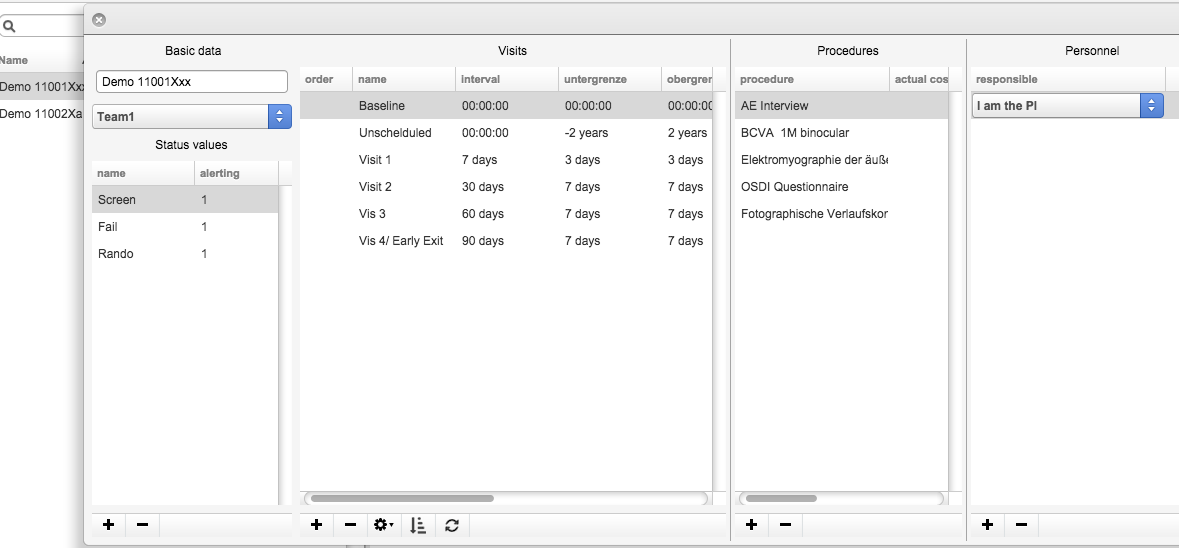
\includegraphics[scale=0.34]{figs/config.png}
\caption{Konfigurationsfenster fŸr die  selektierte Studie. Hier werden u.a. die Statuswerte der fŸr Studienteilnehmer, die Visitenintervalle und deren Prozeduren mit zugehšrigem Personal hinterlegt.}
\label{fig:config}
\end{center}
\end{figure}

\subsection{Grundeinstellungen}
\label{chap:config}
In der ersten Spalte des Konfigurationsfensters lassen sich unter der †berschrift 'Basic data' der Studienname und die GruppenzugehŠrigkeit Šndern. Darunter werden im TableView 'Status values' die ZustŠnde verwaltet, die ein Studienteilnehmer durchlaufen kann. Zu jedem Zustand wird in der Spalte 'alerting' mit einer '1' festgelegt, dass Patienten mit diesem Zustand  kontinuierlich Ÿberwacht werden sollen (z.B. Meldung aller Klinikskontakte via E-Mail). Mit einer '0' wird diese †berwachung unterdrŸckt. Diese Einstellung ist beispielsweise fŸr 'Screen-Failures' oder nach Studienende sinnvoll, um ŸberflŸssige Benachrichtigungen zu vermeiden. Die  E-Mail-Adressen sind im Administrationsbereich hinterlegt (Kapitel \ref{chap:admin}).

\subsection{Visiten}
In der zweiten Rubrik 'Visits' werden die Studienvisiten verwaltet. Jede Visite wird mit dem Plus-Knopf generiert und muss dann geeignet benannt werden. Das jeweilige Visitenintervall wird in die Spalte 'interval' eingetragen. Die Intervalle mŸssen als Zahl mit Einheit eingegeben werden, z.B.  '23 days', '6 mons' oder '2 years'. Toleranzen fŸr den Visitentermin lassen sich Ÿber die beiden  Spalten 'obergrenze' und 'untergrenze' in gleicher weise definieren. Die jeweilige Bezugsvisite fŸr das Visitenintervall muss Ÿber die Spalte 'reference visit' spezifiziert werden. Die einzige Ausnahme bildet die  Referenzvisite (in der Regel die Studieneinschlussvisite). Die Referenzvisite lŠsst sich ggf. Ÿber das Zahnrad-MenŸ 'unset reference visit'  wieder entfernen. Die so markierte Visite wird dadurch  zur Referenzvisite.  Die Visiten lassen sich  Ÿber die Spalte 'ordering' explizit sortieren. Diese Spalte kann mit dem Sortieren-Knopf automatisch belegt werden. In der Spalte 'reimbursement' werden die ausgehandelten VisitenvergŸtungen (in Euro) als einheitslose Zahlen hinterlegt. Diese sind Grundlage fŸr die automatisierte Rechnungserstellung (Kapitel \ref{chap:rechnung}). Die  Kosten einer Visite lassen sich ggf. vorab Ÿber die Visitenprozeduren im Sinne eines Kostenvoranschlages fŸr den Sponsor kalkulieren (s.u.). In der Spalte 'booking' lassen sich die Namen von 'DocsCal'-Sprechstunden hinterlegen, in die Patienten beim Buchen dieser Visite zusŠtzlich zur Studiensprechstunde gebucht werden (beispiel: Fluoreszenangiographie). Die Spallte 'comment' nimmt Kommentare auf, die beim Buchen der Termine eingeblendet werden (Abbildung \ref{fig:visits}).

Zu jeder Visite lassen sich in der Rubrik 'Procedures' des Konfigurationsfensters die zugehšrigen Prozeduren hinterlegen. Prozeduren lassen sich Ÿber den Plus-Knopf hinzufŸgen. Der Eingabefokus springt dann auf die  neue Prozedur und diese kann Ÿber eine ComboBox spezifiziert werden.  Zu jeder Prozedur ist in der Spalte 'base costs' ein Preisvorschlag hinterlegt ('Hauskatalog', Konfiguationsbereich, Kapitel \ref{chap:admin}).  Es muss in der Spalte 'actual costs' ein konkreter Preis festgelegt werden (beispielsweise durch †bernahme des 'base costs'-Wertes). Das bisherige Preisspektrum fŸr diese Prozedur ist in den Spalten 'min' (billigster Preis), 'avg' (durchschnittlicher Preis in allen bisherigen Studien mit dieser Prozedur) und 'max' (bislang hšchster ausgehandelter Preis) sichtbar.
Die Spalten 'ordering' und 'parameter' sind der Gestaltung des elektronischen Worksheets zu dieser Visite vorbehalten (Kapitel \ref{chap:worksheet}). % fixme: what is 'parameter' used for?

In der letzten Rubrik 'Personnel' lassen sich jeder Prozedur eine oder mehrere zustŠndige Personen zuordnen. Die Angabe mehrerer Personen ist dabei als Vertreterkette zu verstehen. Die spezifische Zuordnung von Personen zu Prozeduren ermšglicht zum einen einen personalisierten Kalender (Kapitel \ref{chap:calendar}) als auch eine KonsistenzprŸfung bei der Terminbuchung (Kapitel xx) unter RŸckgriff auf den Abwesenheitskalender (Kapitel \ref{chap:personal}).  Sind alle erforderlichen Personen fŸr die Prozeduren am  avisierten Visitentermin  abwesend, erscheint beim Buchen eine entsprechende   Warnmeldung.

\section{Strukturierte Datenablage}
\label{chap:data}
Die strukturierte Datenablage befindet sich in der Registerkarte 'Eigenschaften'. Sie ermšglicht die  Erfassung frei definierbarer Eigenschaften  fŸr jede Studie am PrŸfzentrum (z.B. Titel, Name des klinischen Monitors usw.). Dabei werden diese Eigenschaften im Sinne eines 'Steckbriefes' stets in der gleichen  Reihenfolge angezeigt. Dies ermšglicht zum das schnelle Auffinden der gesuchten Information, zum anderen werden ausgewŠhlte Datenfelder zum AusfŸllen von hinterlegten Formularen (z.B. Name des Sponsors fŸr die Rechnugserstellung) verwendet. Einige Felder lassen sich direkt Ÿber den 'Play'-Knopf der ButtonBar šffnen. In Tabelle \ref{tab:playbutton} findet sich eine †bersicht  dieser Felder.

\begin{table}[htdp]
\caption{†bersicht Ÿber die Datenfelder, die sich mit dem 'Play'-Knopf der ButtonBar spezifisch šffnen lassen}
\begin{center}
\begin{tabular}{p{4cm}p{8cm}}
Feld & Funktion\\\hline
Monitor Mail  & Bereitet eine Email an den Monitor im EMail-Programm vor\\
NCT-Nummer & Zeigt die registrierten Informationen aus clinicaltrials.gov an\\
Drittmittelnummer & …ffnet die KontoauszŸge dieses Kontos\\
eCRF und IWRS & …ffnet die jeweils hinterlegte URL\\
Serienbrief & Generiert eine PDF-Datei einem Serienbrief (\LaTeX-Format) fŸr alle Studienteilnehmer\\
\end{tabular}
\end{center}
\label{tab:playbutton}
\end{table}%
 
Mit dem Anlegen einer Studie (Kapitel xx) wird eine standardisierte Auswahl aller Datenfelder autmatisch angelegt. Werte lassen sich Ÿber einen Doppelklick auf die Spalte 'val' eingeben bzw. editieren. Wenn lŠngere Texte erfasst werden mŸssen, kann ein mehrzeiliges Eingabefenster Ÿber den Knopf 'Open multiline editor' angefordert werden. Weitere Felder lassen sich Ÿber den Plus-Knopf der ButtonBar ergŠnzen. Es šffnet sich dann eine Auswahlliste, in der eine Mehrfachauswahl mšglich ist, sodass mit einer Aktion mehrere Felder hinzufgefŸgt werden kšnnen (Abbildung xx). In der Auswahlliste lŠsst sich  Ÿber die Spalte 'order' die Reihenfolge der Felder in der strukturierten Datenablage festlegen. Die Spalte 'type' definiert die automatisch angelegten Felder (Wert '1'). In der Spalte 'default' kann ggf. ein Standardwert vorgegeben werden, der bei Anlage des Datenfeldes vorgelegt wird.  †ber die Aktion das Zahnrad-MenŸs der ButtonBar 'add all standard fields' lassen sich fŸr die aktuell markierte Studie alle   Standardfelder erzeugen. Dies ist zum Beispiel sinnvoll, wenn  neue Standardfelder nach dem Anlegen der Studie hinzugefŸgt wurden. Die  Zahnrad-MenŸ-Aktion  'Open annotations...' šffnet ein  Eingabefenster, in dem fŸr jedes Datenfeld beliebige SchlŸssel-Werte Paare  abgelegt werden kšnnen (Abbildung xx). Diese Daten werden fŸr jeden Benutzer getrennt verwaltet und eignen sich daher  zur Ablage von Zugangsdaten. So kšnnen z.B. in dem Feld der URL des eCRF Benutzername und Password in der Annotations-Tabelle hinterlegt werden. Auf diese Weise stehen die Zugangsdaten sicher und ortsunabhŠngig jederzeit zur VerfŸgung. 

\subsection{Volltextsuche}
Das Suchfeld Ÿber der Studientabelle ermšglicht das Durchsuchen der Studien nach Stichwšrtern.  Mehrere Suchbegriffe werden mit dem logischen 'und' verknŸpft. Gro§-/ Kleinschreibung wird ignoriert. Die Suche erfolgt in Echtzeit wŠhrend der Eingabe. Nur  auf die Suchbegriffe zutreffende Studien werden angezeigt. Die Suchbegriffe lassen sich ggf. mit einem Click auf das kleine 'X'  rechts im Suchfeld (Abbildung \ref{fig:search}) eliminieren, um alle Studien wieder anzuzeigen. Bei der Suche werden der Studientitel, alle Felder der strukturierten Datenablage, die Zeitereignisse und das Subject log (Patientennamen / PIZ) berŸcksichtigt. % fixme: <!> dokumente durchsuchen?!.

\begin{figure}[htbp]
\begin{center}
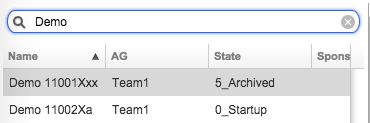
\includegraphics[scale=0.84]{figs/search.png}
\caption{Das Suchfeld Ÿber der Studienliste durchsucht alle Daten in Echtzeit.}
\label{fig:search}
\end{center}
\end{figure}

\subsection{Formulardruck}
Die Felder der strukturierten Datenablage der aktuell selektierten Studie kšnnen in PDF-Formulare und beliebige \LaTeX Vorlagen eingedruckt werden. Momentan sind diesbezŸglich die Dritmittelanzeige sowie ein Anschreiben fŸr den Vertragsumlauf vorbereitet. Beide Formulare lassen sich Ÿber das Zahnrad-MenŸ der ButtonBar unter der Studientabelle abrufen. Weitere  \LaTeX Vorlagen kšnnen hinterlegt werden (Anhang xx). % fixme: <!> das zahnradmenue sollte sich eigentlich automatisch fuellen, sodass ein aufkopieren einer neuen vorlage ausreichen wuerde.


\chapter{Dokumentenablage}
Die Dokumentenablage befindet sich in der Registerkarte 'Dokumente' (Abbildung \ref{fig:docs}). Sie nimmt  beliebige Dokumente  auf. Die Ablage erfolgt fŸr jede Studie getrennt in ca. 20 vorgefertigten Rubriken (z.B. Studienprotokoll, Ethik, Patienteninfo...).  Dokumente kšnnen Ÿber den 'down\-load'-Knopf jederzeit zum Ausdrucken oder zur Ansicht auf die lokale Festplatte kopiert werden (i.d.R. werden PDF und Bilddokumente direkt im Web-Browser angezeigt).

\begin{figure}[htbp]
\begin{center}
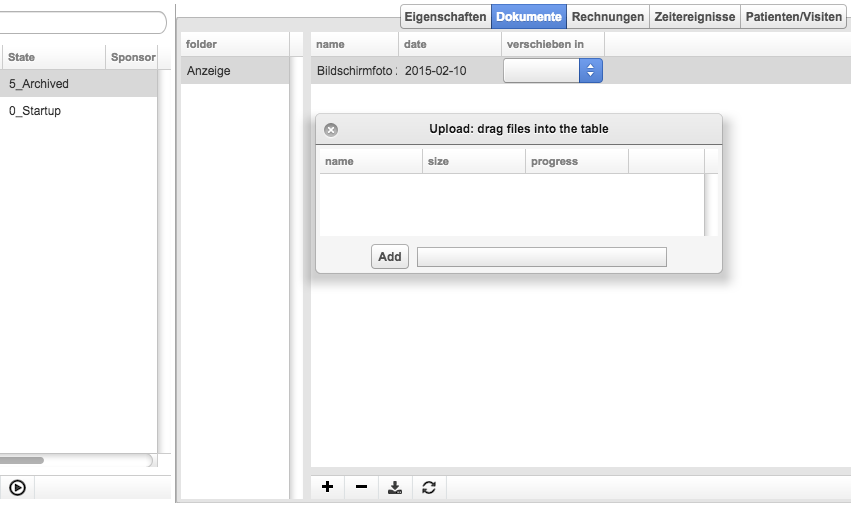
\includegraphics[scale=0.33]{figs/docs.png}
\caption{Dokumentenbereich.}
\label{fig:docs}
\end{center}
\end{figure}


Dateien werden Ÿber den Plus-Knopf der Button-Bar hinzufŸgt. DafŸr šffnet sich das Upload-Fenster (Abbildung xx). Dateien werden der aktuell markierten Studie entweder via Drag-and-Drop in dieses Fenster, oder Ÿber den  'klassischen' Auswahldialog des Betriebssystems hinzugefŸgt. Letzterer lŠsst sich Ÿber den 'Add' Knopf šffnen. Nach dem Upload sind die Dateien  der Rubrike 'Unclassified' zugeordnet. †ber das Popup-MenŸ in der Spalte 'verschieben in' lŠsst sich das Dokument der geeigneten Rubrik zuordnen. Durch einen Doppelklick auf den Dateinamen (Spalte 'name') lŠsst sich der Dateiname editieren. Die Spalte 'date' zeigt das letzte €nderungsdatum der Datei zum Zeitpunkt des Hochladens.

†ber den Minus-Knopf lassen sich Dokumente nach einer SicherheitsrŸckfrage rŸckstandsfrei lšschen. Rubriken ohne zugeordnete Dateien werden nicht angezeigt, sodass ausschlie§lich Rubriken mit zugeordneten Dateien in der Spalte 'folder' gelistet sind. Diese Spalte lŠsst sich ggf. durch BetŠtigen des Reload-Knopfes aktualisieren (beispielsweise nach einem Upload oder nach einer Lšschung).

\chapter{Rechnungswesen}
\label{chap:rechnung}
Das Rechungswesen befindet sich in der Registerkarte 'Rechungen'. Alle Rechnungen der aktuell selektierten Studie sind in dem TableView gelistet. In der Spalte 'creation date' befindet sich das Erzeugungsdatum der Rechnung. Das FŠlligkeitsdatum und ggf. das Datum des Zahlungseinganges finden sich in den beiden Spalten 'due date' und 'date payed'. Diese beiden Spalten ermšglichen  die Funktion 'Download Inkassolist' im HauptmenŸ 'Controlling'. Diese lŠdt eine Excel-Tabelle mit allen ŸberfŠlligen Rechnungen herunter. Die Spalte 'EUR' enthŠlt den Rechungsbetrag in Euro und die Spalte 'comment' einen beliebigen Kommentar zu dieser Rechnung. Die Spalte 'visits ids' beinhaltet eine kommaseparierte Liste der ids aller inkludierten Visiten. Damit wird die Doppelabrechnung von Studienvisiten nachhaltig unterbunden.

Mit dem Plus-Knopf der ButtonBar wird eine einfache leere Rechnung angelegt. Dies eignet sich beispielsweise zur Abrechnung von fixen 'Setup-Fees' u.Š. Die Abrechnung einzelner Visiten ist in den folgenden Kapiteln beschrieben. Der Minus-Knopf lšscht die selektierte Rechnung nach RŸckfrage. Der Download-Knopf generiert die Rechnung im Excel-Format und lŠdt diese zum Ausdrucken herunter.  

\section{Gesamtabrechnung nach Abschluss der Studie}
Die Aktion 'Ausstehende Visiten abrechnen' aus dem ZahnradmenŸ erzeugt eine neue Rechnung Ÿber alle Visitentermine der aktuell selektierten Studie, die bislang noch nicht abgerechnet worden sind. Es werden dabei aber nur Visitentermine aus der Vergangenheit berŸcksichtigt. In die Rechungserstellung flie§en die folgenden Felder aus der strukturierten Datenablage ein:  Name der Studie und Sponsoranschrift , 'Overhead inclusive J/N', 'Umsatzsteuer J/N', 'Drittmittelnummer' und 'Ust-ID'.

\section{Gesamtabrechnung pro Patient}
Sollen einzelne Patienten gezielt abgerechnet werden, mŸssen diese in der Registerkarte 'Patienten/Visits' (Kapitel xx) selektiert werden (eine Mehrfachselektion ist z.B. mit gedrŸckter Shift-Taste mšglich). Anschlie§end wird die entsprechende Rechnung Ÿber die Aktion 'Selektierte Patienten komplett abrechnen' aus dem  Zahnrad-MenŸ der ButtonBar des Patienten-TableViews generiert.

\section{Abrechnung einzelner Visiten}
HŠufig werden Studienvisiten nach der Monitorierung gezielt abgerechnet. Dies lŠsst sich Ÿber die Aktion 'Selektierte Patienten partiell abrechnen' im ZahnradmenŸ der Registerkarte 'Patienten/Visits' (Kapitel xx) erreichen. Es šffnet sich das zweispaltige Fenster 'Einzelvisiten abrechnen' (Abbildung xx). In der linken Spalte sind alle Rechnungen der aktuellen Studie gelistet.  In der linken Spalte sind alle durchgefŸhrten Visiten des aktuellen Patienten aufgelistet. Nun muss in der rechten Spalte Die Rechnung, Ÿber die die Visiten abgerechnet werden sollen, selektiert werden.  †ber die Plus-Taste lŠsst sich ggf. dafŸr eine neue 'leere' Rechnung erzeugen. Als nŠchstes mŸssen die abzurechnenden Visiten markiert werden (mit gedrŸckter Maustaste Ÿber die Visiten 'ziehen' bzw. mit gedrŸckter Shift- bzw. Kommando-Taste mehrfach klicken). Abschlie§end werden diese Visiten dann Ÿber die Zahnrad-Aktion 'Selektierte abrechnen' der ButtonBar unter dem Visiten-TableView des Fensters 'Einzelvisiten abrechnen' in die selektierte Rechnung einbezogen.

\section{Fahrtkostenabwicklung}
Fahrtkosten werden Ÿblicherweise von dem PrŸfzentrum vorgestreckt. †ber  die Aktion 'Fahrtkosten erstatten' im ZahnradmenŸ der Registerkarte 'Patienten/Visits' (Kapitel xx) lŠsst sich eine Auszahlanordnung fŸr die Fahrtkosten einzelner Visiten generieren und die Auszahlung zwecks RŸckvergŸtung durch den Sponsor dokumentieren. Es šffnet sich ein Fenster mit dem Titel 'Fahrtkostenerstattung' (Abbildung xx). In die Felder 'IBAN' und 'BIC' lassen sich ggf. jeweils die 'alte' Kontonummer und Bankleitzahl eintragen. †ber die Zahnrad-Aktion 'Validate IBAN' werden diese in IBAN und BIC umgerechnet. Die Bank wird Ÿber eine lokale Datenbank automatisch aus der IBAN abgeleitet. War bereits eine IBAN eingetragen, erfolgt eine PrŸfung IBAN PrŸfziffer, und es wird bei Inkonsistenzen ggf. eine Warnmeldung ausgegeben.  In das Feld 'Travel distance' wird bereits mit dem …ffnen des Fensters  die Anreisedistanz mittels PKW eingetragen (Hin- und RŸckreise gemŠ§ Google-Maps-API). Aus DatenschutzgrŸnden wird dabei nicht die volle Adressinformation Ÿbermittelt, sodass die Distanz geringfŸgig von einer manuellen Suche in 'Google-Maps' abweichen kann. Die Fahrtkosten werden durch eine Multiplikation der Anreisedistanz mit der vertraglich vereinbarten Kilometerpauschale ermittelt (Feld '' in der strukturierten Datenablage, Kapitel xx).

In der Spalte 'date' findet sich das Visitendatum. In der Spalte 'add. costs' lassen sich ggf. Zusatzkosten zu dem o.g. Kilometergeld (z.B. ParkgebŸhren) fŸr die jeweilige Visite geltend machen. In die Spalte 'alt. costs' kann ggf. ein alternativer Festpreis fŸr die An- und Abreise zu dieser Visite festgelegt werden (beispielsweise Taxikosten oder Preis des Bahntickets). Die Spalte 'date reimbursed' nimmt das Abrechnungsdatum auf. Dieses merkt den Fahrtkostenbetrag schlussendlich fŸr die spŠtere RŸckvergŸtung durch den Sponsor vor und wird Ÿber die Zahnradaktion 'Als abgerechnet markieren' automatisch eingetragen. Die Spalte Kommentar nimmt ggf. einen begrŸnden Text auf, der  auf das Anordnungsformular Ÿbernommen wird.

\chapter{Termine und Ereignisse}
Das Zeitereignisse der aktuell selektierten Studie werden  unter der Registerkarte 'Zeitereignisse' verwaltet. Ein neues Ereignis kann Ÿber den Plus-Knopf der Button-Bar  angelegt werden.   Danach muss Ÿber das Popup der Spalte 'name' die Bedeutung des Ereignisses definiert werden.  Start- und Enddatum kšnnen Ÿber einen Doppelklick in die Spalten 'start' und 'end' eingegeben oder Ÿber einen Minikalender ausgewŠhlt werden. FŸr Ereignisse, die noch nicht abgeschlossen bzw. erledigt sind, kann das Enddatum auch ausgelassen werden. Die Spalte 'responsible' nimmt ggf. die zustŠndige Person auf, und in der Spalte 'comment' kann erklŠrender Freitext abgelegt werden.
\section{Aufgabenlisten}
Die Zeitereignisse dienen zum einen dazu, Meilensteine oder Treffen (z.B. Monitorierung oder Initiierungen) in den Arbeitskalender einzutragen. Zeitereignisse kšnnen zum anderen als Aufgabenlisten fungieren (z.B. Schulungen fŸr einzelne Personen). In diesem Fall darf  erst nach Absolvierung der Aufgabe ein geeignetes Datum in die Spalte 'end' eingetragen werden. †ber die Zahnradaktion 'Todo liste' lŠdt eine Excel-Tabelle mit allen nicht erledigten Aufgaben der aktuellen Studie herunter. Der Befehl 'Download Todo Liste'  aus dem 'Controlling'-HauptmenŸ generiert eine Gesamtliste der noch nicht erledigten Aufgaben in allen Studien, die dem aktuellen Benutzer zugeordnet sind.

\section{Studienzustand}
\label{section:zyklus}
Die Zeitereignisse definieren zudem indirekt den aktuellen Zustand im 'Lebenszyklus der Studie', der in der Spalte 'State' der linken StudienŸbersicht erscheint. Alle mšglichen ZustŠnde sind in Tabelle \ref{tab:trialstates} zusammen gefasst.

\begin{table}[htdp]
\caption{†bersicht Ÿber alle ZustŠnde, die jede Studie Ÿber die Zeit durchlŠuft}
\begin{center}
\begin{tabular}{p{4cm}p{8cm}}
Name & Bedeutung \\\hline
Upcoming  & Das Anfangsdatum des Ereignisses Gesamtlaufzeit liegt in der Zukunft.\\
Startup & Das Anfangsdatum des Ereignisses Gesamtlaufzeit wurde bereits Ÿberschritten, das Anfangsdatum des Ereignisses Rekrutierung liegt aber noch in der Zukunft.\\
Recruiting & Anfangsdatum des Ereignisses Rekrutierung wurde Ÿberschritten und das Enddatum noch nicht erreicht.\\
Follow up & Das Enddatum des Ereignisses Rekrutierung wurde Ÿberschritten und das Enddatum des Ereignisses Gesamtlaufzeit wurde noch nicht erreicht.\\
Finished & Das Enddatum des Ereignisses Gesamtlaufzeit wurde Ÿberschritten.\\
Archived & Das Enddatum des Ereignisses Gesamtlaufzeit wurde Ÿberschritten und das Feld 'Aufbewahrung bis' wurde in der strukturierten Datenablage angelegt (Kapitel xx)\\
\end{tabular}
\end{center}
\label{tab:trialstates}
\end{table}

\section{Arbeitskalender}
\label{chap:calendar}
Das Kalenderfenster šffnet sich Ÿber das 'Special'-HauptmenŸ  (Abbildung xx). Es wird der aktuelle Monat angezeigt und der aktuelle Tag  gelb umrandet. Andere Jahre und Monate kšnnen Ÿber die beiden ersten Eingabefelder oberhalb des Kalenderbereiches ausgewŠhlt werden.
Studienvisiten sind in schwarzer, andere Ereignisse wie beispielsweise Monitorierungsvisiten, Teameetings (Kapitel xx) oder Personalabwesenheiten (Kapitel xx) in  grauer Schrift dargestellt. Termine mit †berschneidungen oder Konflikten sind mit einem Ausrufungszeichen in spitzen Klammern gekennzeichnet.

 Die   Ereignisse kšnnen Ÿber das Ankreuzfeld 'Filter for me'  fŸr  den aktuellen Benutzer gefiltert werden. Dies blendet alle Studienvisiten aus, bei denen der aktuelle Benutzer keiner Prozedur (Kapitel xx)  zugeordnet ist. ZusŠtzlich werden die Zeitereignisse, die explizit einer anderen Person zugewiesen sind nicht mehr angezeigt.  Der Kalender steht unter der URL /iCAL/{\it ldap} auch als iCAL feed zur VerfŸgung ({\it ldap}  muss selbstverstŠndlich durch das eigene LDAP-KŸrzel ersetzt werden ). †ber die Parameter '?personalized=1' kann der Feed analog zum  Ankreuzfeld 'Filter for me' personalisiert werden. % stimmt der link?! parameter show end dokumentieren.
Team meetings.





\chapter{Patienten und Visiten}
\section{Patienten}
Die Liste der Studienpatienten bzw. das 'Subject identification log'   ist unter der Registerkarte 'Patienten/Visiten' angeordnet. Neue Patienten werden Ÿber den Plus-Knopf unter der Patiententabelle angelegt. Der Eingabefokus bewegt sich damit  direkt in das Feld fŸr die 'Personenidentifikationsziffer' ('PIZ'). Nach Eingabe einer  PIZ werden mit dem BetŠtigen der Eingabetaste die Felder 'name', 'givenname' und 'birthdate' automatisch aus dem Klinik-Informationssystem Ÿbernommen. Auch die Anschrift ist hinterlegt (beispielsweise fŸr die Serienbrieffunktion, \ref{tab:playbutton}).

Die Spalte 'state' ermšglicht die Zuordnung eines vordefinierten Statuswertes (Studienkonfiguration, Kapitel \ref{chap:config}). Dadurch wird beispielsweise festgelegt, ob der Studienteilnehmer elektronisch 'Ÿberwacht' werden soll. In diesem Fall werden  E-Mails verschickt, wenn der Patient (auch ungeplant) im Klinikum vorstellig wird. Dies hilft beispielsweise dabei 'Severe adverse events'  fristgerecht zu melden. Die Spalten 'code1' und 'code2' nehmen ggf. studienspezifische Pseudonymisierungsdaten auf. In die Spalte 'comment' lŠsst sich ein beliebiger Text zu dem Patienten hinterlegen. Das ist beispielsweise sinnvoll, um den Grund fŸr ein 'Screen-Failure' zu dokumentieren. †ber den Download-Knopf in der ButtonBar lŠsst sich die Patientenliste als Excel-Datei herunterladen. In dieser Tabelle ist auch das EinfŸgedatum vermerkt. Diese Datei kann ggf. als 'Subject identification log' ausgedruckt oder in elektronische Formulare des Sponsors einkopiert werden. Nach Entfernen der Klarnamen lŠsst sich diese Tabelle  als Screening log verwenden.

†ber die Zahnradknopf-Aktion 'Brief an Hausarzt' wird ein Brief an den Hausarzt generiert, der Ÿber die Studienteilnahme des aktuellen Patienten informiert. Die  Zahnradaktionen zur Abrechnung sind in Kapitel \ref{chap:rechnung} beschrieben. Die Aktion 'Open DCV' šffnet die digitale Akte des aktuellen Patienten.

\section{Visiten}
Die Visiten des aktuellen Patienten befinden sich in der Tabelle rechts daneben (Abbildung \ref{fig:visits}). Die Visiten werden mit der Neueingabe jedes Patienten automatisch angelegt. †ber den Plus-Knopf kšnnen ggf. zusŠtzliche Visiten angelegt werden (beispielsweise im Falle ungeplanter Kontrollen). Nicht mehr benštigte Visiten kšnnen Ÿber den Minus-Knopf gelšscht werden. †ber die Zahnradknopf-Aktion 'Create all visits' lassen sich  alle momentan noch fehlenden Visiten ergŠnzen. Dies ist beispielsweise sinnvoll, wenn seit Anlage des Patienten neue Studienvisiten in der Studienkonfigurationsmaske (Kapitel  \ref{chap:config}) erŠnzt wurden. Die Visite wird Ÿber die Spalte 'visit' Ÿber ein Popup-MenŸ spezifiziert.

\begin{figure}[htbp]
\begin{center}
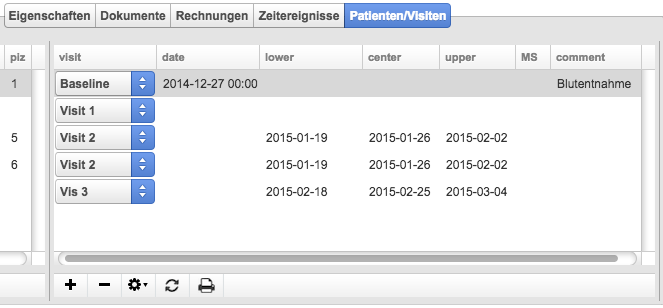
\includegraphics[scale=0.63]{figs/visits.png}
\caption{Visitentabelle des aktuellen Patienten.}
\label{fig:visits}
\end{center}
\end{figure}

Die Spalte 'date' nimmt das Datum der Visite auf. Dieses ist fŸr die Referenzvisite mit dem Tagesdatum bei Neuanlage vorbelegt. †ber einen Doppelklick kann das Datum manuell editiert bzw. aus einem Popup-Mini-Kalender ausgewŠhlt werden. Dabei sind die Dati au§erhalb der Visitenfenster ausgegraut. Die Datumsgrenzen des Visitenfenster sind in den Spalten 'lower' und 'upper' angezeigt. Die Spalte 'center' zeigt den optimalen Termin. Diese Datumswerte errechnen sich aus dem Einschlussdatum, also dem Datumswert der Referenzvisite. Mit €nderung dieses Datums bzw. €nderung der Visitenintervalle (Kapitel  \ref{chap:config}) lassen sich die Visitenfenster Ÿber den  'Reload'-Knopf aus der ButtonBar neu berechnen. Sind die Datumswerte fŸr die Visitenfenster leer, ist in der Regel die Referenzvisite noch nicht terminiert.

Dabei erfolgt im Hintergrund zusŠtzlich ein Abgleich mit den Terminen der zugehšrigen Sprechstunde (Einstellung s. Kapitel xx). Ist innerhalb eines Visitenfensters kein buchbarer Terminen mehr vorhanden, wird in der Spalte 'MS' ein Warndreieck eingeblendet (dies kann bei hoher Auslastung des Buchungssystems des Klinikums ggf. einige Sekunden dauern). Diese Funktion ist beispielsweise fŸr engmaschig getaktete Studien mit geringen Toleranzen hilfreich um zu entscheiden, ob in AbhŠngigkeit vom Einschlussdatum Visitentermine auf das Wochenende fallen wŸrden.

In die Spalte 'comment' wird das Kommentarfeld zu dieser Visite aus dem Konfigurationsfenster eingeblendet. Alle in der Visitentabelle dargestellten Informationen lassen sich Ÿber den Drucken-Knopf auf einen Terminzettel drucken, der dem Patienten ausgehŠndigt werden kann.

Die Patienten kšnnen Ÿber die Tabelle rechts neben den Visiten mittels Doppelklick in das Order-Entry-System des Klinikums eingebucht werden. Studien- und Visitenname werden als Buchungstext vorgeschlagen und kšnnen ggf. ergŠnzt werden. Mit dem Knopf-Buchen erfolgt die Buchung, was  ggf. einige Sekunden dauern kann (erkennbar an dem Drehrad). Bei erfolgreicher Buchung wird der gebuchte Termin fŸr die selektierte Visite  eingetragen. Dann erfolgt im Hintergrund eine †berprŸfung dieser Buchung auf etwaige TerminŸberschneidungen. DafŸr werden die Terminkalender aller fŸr die Abwicklung der Visitenprozeduren Personen auf Grundlage der hinterlegten DurchfŸhrungszeitrŠume ŸberprŸft. †berschneidet sich fŸr mindestens eine Person der aktuelle Termin mit bereits gebi

% Open/print worksheet, , dummy for booking. Ÿberschneidungen.
\section{Worksheets}
\label{chap:worksheet}

\chapter{HauptmenŸ}
\section{Edit}
\section{Controlling}
\section{Special}


\chapter{Persšnlicher Bereich}
\label{chap:personal}
Wie kommt man hin, wie trŠgt man termine ein, wie trŠgt man teilzeit ein (abwesenheit an einzelnen tagen). Download Visitconflictlist erklaeren.


\chapter{Administrationbereich}
\label{chap:admin}
Hier werden globale eigenschaften hinterlegt.
\section{Benutzerverwaltung}
ErklŠrung des Rechtekonzepts.
Das Programm unterstŸtzt mehrere Arbeitsgruppen. Jeder Benutzer ist mindestens einer Arbeitsgruppe zugeordnet. Nur die Studien  der zugeordneten Arbeitsgruppen sind fŸr den angemeldeten Benutzer sichtbar. Die Benutzerverwaltung und das Rechte\-konzept sind in Kapitel xx dargestellt.

\section{Team Meetings}
Wie kommt man hin, wie trŠgt man termine ein, wie trŠgt man teilzeit ein (abwesenheit an einzelnen tagen). Download Visitconflictlist erklaeren.


ErklŠrung der einzelnen Tabs.
\section{Groupware features}

\section{Prozedurenkatalog}
Hauspreise, GoAE
Verweis auf Anhang mit beispielcode. Dauer der prozedur in minuten..

\begin{appendix}

\chapter{Erstellung eigener Widgets}
Klassenhierachie, SimpleWidget vs. Cappusance, Timer, Stopwatch.

\begin{lstlisting}[caption=Complete source code of a minimalistic widget.,  label= lst:form, basicstyle={\small\ttfamily}, numbers=left]
<?xml version="1.0"?>
<!DOCTYPE gsmarkup>
<gsmarkup>
  <objects>
Ê  <window visible="NO">
Ê Ê  <hbox id="widgets">
Ê Ê Ê Ê Ê Ê<label valign="center"> Haben sich SAEs ereignet?</label>
Ê Ê Ê Ê Ê Ê<popUpButton width="80" valueBinding="#CPOwner.value2">
Ê Ê Ê Ê Ê Ê Ê Ê <popUpButtonItem title="Ja" tag="1"/>
Ê Ê Ê Ê Ê Ê Ê Ê <popUpButtonItem title="Nein" tag="0"/>
Ê Ê Ê Ê Ê Ê</popUpButton>
Ê Ê Ê Ê Ê <label valign="center"> Zeit </label>
Ê Ê Ê Ê Ê <textField valueBinding="#CPOwner.value1" width="120" halign="min"/>
Ê Ê Ê Ê Ê <button title="Notieren" target="#CPOwner" action="takeTime:"/>
Ê   </hbox>
   </window>
  </objects>
  <connectors>
  Ê Ê<outlet source="#CPOwner" target="widgets" label="_myView"/>
  </connectors>
</gsmarkup>}
\end{lstlisting}

\begin{lstlisting}[caption=Corresponding LaTeX template.,  label= lst:form, basicstyle={\small\ttfamily}, numbers=left]
{{\bf<value2>} (0=Nein, 1=Ja). Beantwortet: {\bf<value1>}}
\end{lstlisting}
\chapter{Erstellung eigener Formulare}

\chapter{Installationsanleitung}

\begin{lstlisting}[caption=Installationsbefehle beispielhaft fuer MacOS X.,  label= lst:form, basicstyle={\small\ttfamily}, numbers=left]
# the easiest way to get Postgres up and running on a mac is Postgres.app
/Applications/Postgres.app/Contents/Versions/9.3/bin/createdb  aug_clinical
/Applications/Postgres.app/Contents/Versions/9.3/bin/createuser postgres -s
/Applications/Postgres.app/Contents/Versions/9.3/bin/createuser root -s
cat sql_template.sql | /Applications/Postgres.app/Contents/Versions/9.3/bin/psql aug_clinical
#
# we need a current TeX distribution such as <https://tug.org/mactex/>
# perl is already installed on linux and mac but we need quite a bunch of non-core perl modules
sudo perl -MCPAN -e 'install ($_) for qw/Mojolicious Mojolicious::Plugin::Database Mojolicious::Plugin::RenderFile SQL::Abstract::More Apache::Session::File Spreadsheet::WriteExcel Spreadsheet::ParseExcel Business::IBAN DBD::Pg Date::ICal Data::ICal Data::ICal::Entry::TimeZone/'
# now you can either call morbo backend.pl (testing server)
# or launch hypnotoad backend.pl during system boot
# locate your favourite web browser to http://localhost:3000/Frontend/index.html
# (you may change the port either in backend.pl or from the command line)
# the username is pi with no password
# (passwords are not enforced unless you modify the helper LDAPChallenge with backend.pl appropriately)
\end{lstlisting}

\chapter{Danksagungen}

\begin{itemize}
\item Cappuccino Project
\item FontAwesome

\end{itemize}

\end{appendix}

\end{document}
